\documentclass[12pt]{amsart}
\usepackage{fullpage}
\makeatletter

%% AMS
\usepackage{amsmath,amssymb,latexsym}

%% Theorems
\usepackage{xcolor}
\definecolor{darkgreen}{rgb}{0,0.45,0} 
\usepackage[pagebackref,colorlinks,citecolor=darkgreen,linkcolor=darkgreen]{hyperref}
\usepackage{cleveref,aliascnt}
\usepackage{amsthm}
\def\defthm#1#2#3{%
  %% Ensure all theorem types are numbered with the same counter
  \newaliascnt{#1}{thm}
  \newtheorem{#1}[#1]{#2}
  \aliascntresetthe{#1}
  %% Tell cleveref's \cref what to call things
  \crefname{#1}{#2}{#3}}
\newtheorem{thm}{Theorem}[section]
\crefname{thm}{Theorem}{Theorems}
\theoremstyle{definition}
\defthm{defn}{Definition}{Definitions}
%\theoremstyle{remark}
\defthm{rmk}{Remark}{Remarks}
\defthm{advrmk}{Advanced Remark}{Advanced Remarks}
\newenvironment{adv}{\small\begin{advrmk}}{\end{advrmk}}
\defthm{eg}{Example}{Examples}
\defthm{egs}{Examples}{Examples}
\defthm{sage}{Sage}{Sages}

%% Reference format for sections
\crefformat{section}{\S#2#1#3}
\Crefformat{section}{Section~#2#1#3}
\crefrangeformat{section}{\S\S#3#1#4--#5#2#6}
\Crefrangeformat{section}{Sections~#3#1#4--#5#2#6}
\crefmultiformat{section}{\S\S#2#1#3}{ and~#2#1#3}{, #2#1#3}{ and~#2#1#3}
\Crefmultiformat{section}{Sections~#2#1#3}{ and~#2#1#3}{, #2#1#3}{ and~#2#1#3}
\crefrangemultiformat{section}{\S\S#3#1#4--#5#2#6}{ and~#3#1#4--#5#2#6}{, #3#1#4--#5#2#6}{ and~#3#1#4--#5#2#6}
\Crefrangemultiformat{section}{Sections~#3#1#4--#5#2#6}{ and~#3#1#4--#5#2#6}{, #3#1#4--#5#2#6}{ and~#3#1#4--#5#2#6}

%% Use the theorem counter for equations as well
\let\c@equation\c@thm
\numberwithin{equation}{section}

%% Pictures
\usepackage{tikz}
\usepackage{graphicx}

%% Differentials
\newcommand{\dd}{\ensuremath{\mathrm{d}}}
\newcommand{\ed}{\ensuremath{\mathrm{d}\wedge}}

%% Differentials of variables
\newcommand{\dx}{{\ensuremath{\dd x}}}
\newcommand{\dy}{{\ensuremath{\dd y}}}
\newcommand{\dz}{{\ensuremath{\dd z}}}
\newcommand{\dzbar}{{\ensuremath{\dd \bar{z}}}}
\newcommand{\dt}{{\ensuremath{\dd t}}}
\newcommand{\du}{{\ensuremath{\dd u}}}
\newcommand{\dv}{{\ensuremath{\dd v}}}
\newcommand{\df}{{\ensuremath{\dd f}}}
\newcommand{\dg}{{\ensuremath{\dd g}}}
\renewcommand{\dh}{{\ensuremath{\dd h}}}
\newcommand{\dr}{{\ensuremath{\dd r}}}
\newcommand{\drho}{{\ensuremath{\dd \rho}}}
\newcommand{\dtheta}{{\ensuremath{\dd \theta}}}
\newcommand{\dphi}{{\ensuremath{\dd \phi}}}
\newcommand{\dpx}{{\ensuremath{\dd \pt{x}}}}

%% Not differentials of anything
\usepackage[T1]{fontenc}
\usepackage{lmodern}
\newcommand{\dl}{\ensuremath{\mathrm{\dj}\ell}}
\newcommand{\dA}{\ensuremath{\mathrm{\dj}A}}
\newcommand{\dV}{\ensuremath{\mathrm{\dj}V}}
\newcommand{\dn}{\ensuremath{\mathrm{\dj}\vc{n}}}

%% Wedge product
%\newcommand{\wedge}{\wedge}

%% Partial derivatives
% \newcommand{\pder}[2]{\frac{\partial #1}{\partial #2}}
% \newcommand{\pdertwo}[2]{\frac{\partial^2 #1}{\partial #2^2}}
% \newcommand{\pdermixed}[3]{\frac{\partial^2 #1}{\partial #2 \,\partial #3}}
\newcommand{\pder}[2]{{#1}_{#2}}
\newcommand{\pdertwo}[2]{{#1}_{{#2}{#2}}}
\newcommand{\pdermixed}[3]{{#1}_{{#2}{#3}}}

%% Transposing vectors into forms
\newcommand{\tr}[1]{{#1}^\top}
\newcommand{\ptr}[1]{{(#1)}^\top}

%% Hodge star on forms
\newcommand{\str}[1]{{#1}^*}
\newcommand{\pstr}[1]{{(#1)}^*}

%% Points and vectors
\newcommand{\pt}[1]{\mathbf{#1}}
\newcommand{\ptc}[1]{(#1)}
\newcommand{\ptx}{\pt{x}}
% \newcommand{\vc}[1]{\vec{#1}}
\newcommand{\vc}[1]{\mathbf{#1}}
\newcommand{\vcc}[1]{(#1)}
\newcommand{\lrvcc}[1]{\left(#1\right)}

%% Vector operations
\newcommand{\mgn}[1]{\Vert #1 \Vert}
%\newcommand{\dotp}[2]{\langle #1 , #2 \rangle}
\newcommand{\dotp}[2]{#1 \cdot #2}
\newcommand{\crossp}[2]{#1 \times #2}

%% Vector calculus operations
\newcommand{\grad}[1]{\nabla #1}
\renewcommand{\div}[1]{\nabla \cdot #1}
\newcommand{\curl}[1]{\nabla \times #1}

%% Fractions
\newcommand{\half}{\ensuremath{\textstyle\frac{1}{2}}}
\newcommand{\halfi}{\ensuremath{\textstyle\frac{1}{2i}}}
\newcommand{\halfpii}{\ensuremath{\textstyle\frac{1}{2\pi i}}}
\newcommand{\third}{\ensuremath{\textstyle\frac{1}{3}}}

%% Orders
\renewcommand{\th}{^{\mathrm{th}}}
\newcommand{\st}{^{\mathrm{st}}}

%% Approximation to specified order
\newcommand{\apx}[1]{\mathrel{\overset{#1}{\approx}}}

%% Riemann sums
\newcommand{\rstag}[2]{{#1}_{#2}^*}

%% Complex conjugation
\newcommand{\conj}[1]{\bar{#1}}
\newcommand{\zbar}{\conj{z}}
\newcommand{\wbar}{\conj{w}}

%% Parametrized curves
\newcommand{\curve}{C}
\newcommand{\curvept}{\mathbf{x}}
\newcommand{\dcurvept}{\dd\mathbf{x}}
\newcommand{\curvex}{x}
\newcommand{\curvey}{y}
\newcommand{\curvez}{z}

%% Regions
\newcommand{\region}{R}
\newcommand{\bdry}{\partial}

%% Parametrized surfaces
\newcommand{\surf}{S}
\newcommand{\surfx}{x}
\newcommand{\surfy}{y}
\newcommand{\surfz}{z}

%% Integrals of differential forms.  The only argument is the
%% integration manifold; the differential form just comes afterwards.
\newcommand{\lint}[1]{\int_{#1}} % line integral over a curve
\newcommand{\sint}[1]{\iint_{#1}} % surface integral form over a surface
\newcommand{\vint}[1]{\iiint_{#1}} % volume integral over a spatial region

%% "Classical" integrals.  For these the integrand is a *function*
%% (well, technically, an expression with free variables) which is
%% given as a second argument.
\newcommand{\dint}[2]{\iint_{#1} #2 \,\dA} % double integral over a plane region
\newcommand{\tint}[2]{\iiint_{#1} #2 \,\dV} % triple integral over a spatial region
\newcommand{\itint}[4]{\int_{#2}^{#3} #4 \,\dd #1} % ordinary one-variable integral over an interval
\newcommand{\itdint}[7]{\int_{#2}^{#3} \int_{#5}^{#6} #7 \,\dd #4\,\dd #1} % double iterated integral
% Can't have more than 9 parameters
%\newcommand{\ittint}[10]{\int_{#2}^{#3} \int_{#5}^{#6} \int_{#8}^{#9} #10 \,\dd #7\,\dd #4\,\dd #1} % triple iterated integral
\makeatletter
\newcommand{\ittint}[3]{\int_{#2}^{#3} \@ittint #1}
\newcommand{\@ittint}[8]{\int_{#3}^{#4} \int_{#6}^{#7} #8 \,\dd #5\,\dd #2\,\dd #1} % triple iterated integral
\makeatother

%% Textbooks
\usepackage{version}
\includeversion{notextbook}
\excludeversion{stewart}
\excludeversion{hugheshallett}
\excludeversion{rogawski}

\makeatother

\title{On differential forms}
\begin{document}
\maketitle

In your previous calculus classes, you may or may not have encountered \emph{differential forms} by name.
However, you've certainly met them, even if you didn't realize it.
When you write
\[ \int_{x=a}^b f(x) \,\dx \]
the thing being integrated, ``$f(x) \,\dx$'', is a differential form.

You may have been told that the ``$\dx$'' is simply a notation that indicates which variable we're integrating, but this is a lie.
In multivariable calculus, we can no longer maintain this fiction: we have to treat differential forms as honest objects.
Fortunately, we also have two advantages over one-variable calculus in understanding differential forms: we have \emph{vectors} at our disposal; and some things are actually \emph{less} confusing in more dimensions because there are fewer coincidences to get confused by.

\section{Differential forms}
\label{sec:differential-forms}

If $\dx$ isn't just a notation indicating the integration variable, what is it?
If you encountered differentials in one-variable calculus, you may have been told that $\dx$ is a small change in $x$ (sometimes denoted $\Delta x$), or even an ``infinitesimal'' change in $x$.
These are not wrong, but with vectors we can give a better definition.

\begin{defn}
  A \textbf{differential 1-form} is a function whose input is a point $\pt{x}$ \emph{and} a vector based at $\pt{x}$.
  We denote the vector by $\dpx$.
\end{defn}

In $n$ dimensions, the point $\pt{x}$ has $n$ coordinates, as does the vector $\dpx$.
As usual, in 2 or 3 dimensions we denote the coordinates of $\pt{x}$ by $\ptc{x,y}$ or $\ptc{x,y,z}$.
Similarly, we denote the coordinates of $\dpx$ by $\vcc{\dx,\dy}$ or $\vcc{\dx,\dy,\dz}$.
We can then describe a differential form by a formula involving these coordinates $x,y,z,\dx,\dy,\dz$.

We usually denote differential forms by lowercase Greek letters such as $\omega$ (omega, not to be confused with the English letter $w$) or $\eta$ (eta, not to be confused with the English letter $n$).
Thus we would write $\omega(\pt{x},\dpx)$ for the value of a form $\omega$ at a point $\pt{x}$ and a vector $\dpx$, or $\omega(x,y,\dx,\dy)$ if we want to emphasize all the coordinates.

\begin{egs}\label{egs:differential-forms}
  The following are all differential 1-forms:
  \begin{gather*}
    x^2 \,\dx + 2xy \, \dy\\
    \half({x-z}) \,\dx - 4\, \dy + e^y \,\dz\\
    1 + \dx + \half \dx^2 + \third \dx^3\\
    \sin(x + \dx) - \sin(x)\\
    \sqrt{\dx^2+\dy^2}
  \end{gather*}
\end{egs}

Note that although $\dx$ is two letters, we regard it as one symbol standing for one variable.
In particular, an expression such as $\dx^2$ means $(\dx)^2$, not $\dd(x^2)$.
(We will give a different meaning to $\dd(x^2)$ in \cref{sec:differentials}.)

The first two of \cref{egs:differential-forms} are special in the following way.

\begin{defn}
  A \textbf{linear} differential 1-form is one defined by an expression such as
  \[ f(\pt{x}) \, \dx + g(\pt{x}) \, \dy + h(\pt{x}) \, \dz. \]
  Here $f$, $g$, and $h$ are functions of the point $\pt{x}$ only, and each of them is multiplied by one of the coordinates of $\dpx$.
\end{defn}

Most mathematicians only use the term ``differential 1-form'' for linear ones.
However, the more general ones are quite useful.

It is helpful to think of the coordinates $\dx$, $\dy$, and $\dz$ as small changes in the value of $x$.
For instance, if $x=3$, then a possible small change would be $\dx = 0.01$.
In this case, a differential form such as $\dx^2$ is an \emph{even smaller} change, since $\dx^2 = 0.0001$.
We say that $\dx$ is a \emph{first order} form while $\dx^2$ is \emph{second order}.
Similarly, we say that $x$ itself is \emph{zeroth order}, as is any function value $f(\pt{x})$ not involving $\dpx$.

Every linear form is first-order: when we multiply a zeroth order number like $f(\pt{x})$ by a first order one like $\dx$, the result is first order.
For instance, if $f(x) = 4$ and $\dx = 0.001$, then $f(x)\,\dx = 0.004$.

The concept of order can be applied even to forms that are not polynomials in $\dx$.
For instance, if $\dx=0.01$, then $\sin \dx \approx 0.0099998$, which is about the same size as $\dx$.
Thus, it is reasonable to say that $\sin\dx$ is also first-order.
On the other hand, still with $\dx=0.01$, we have $\cos \dx - 1 \approx -0.00005$, which is much smaller than $\dx$ and about the same size as $\dx^2$.
Thus, it is reasonable to say that $\cos \dx - 1$ is second-order.

We make the notion of ``orders'' precise with the following definition.

\begin{defn}
  Let $n$ be an integer $\ge 0$.
  A 1-form $\omega$ is \textbf{$n\th$ order} at a point $\pt{x}$ if
  \[ \lim_{\dpx\to 0} \frac{\omega(\pt{x},\dpx)}{\mgn{\dpx}^{n-1}} = 0 \]
  for all vectors $\dpx$ based at $\pt{x}$.
\end{defn}

Recall that definitions in mathematics introduce a \emph{new} meaning for a word.
Thus, \emph{from now on} (in this class) the word ``order'' \emph{will mean} what this definition says it does.
Our previous discussion was only motivational; the definition is the ``gold standard'' for the meaning of the word.

The first thing to do in understanding a definition is to look at some examples.
If we chose the definition well, the examples will justify our motivation.

\begin{eg}
  As suggested above, any continuous \emph{linear} differential 1-form is first order at every point.
  For instance, if $\omega(\pt{x},\dd\pt{x}) = f(\pt{x}) \, \dx$, then
  \[ \frac{\omega(\pt{x},\dpx)}{\mgn{\dpx}^0} = f(\pt{x}) \, \dx\]
  which goes to zero as $\dx\to 0$ (for fixed $\pt{x}$).
\end{eg}

\begin{eg}
  \emph{Any} continuous differential 1-form is zeroth order at every point.
  For since $\frac{1}{h^{-1}} = h$, we have
  \[\frac{\omega(\pt{x},\dpx)}{\mgn{\dpx}^{-1}} = \mgn{\dpx} \, \omega(\pt{x},\dpx).\]
  Since $\omega$ is continuous, $\lim_{\dpx\to 0} \omega(\pt{x},\dpx)$ exists; while of course $\lim_{\dpx\to 0} \mgn{\dpx} = 0$.
  Thus, by the product law for limits, the limit of the product is also zero.
\end{eg}

\begin{eg}
  The differential form $\dx^2$ is second order at any point.
  We have
  \[ \frac{\omega(\pt{x},\dpx)}{\mgn{\dpx}^1} = \frac{(\dx)^2}{\dx} = \dx \]
  which of course goes to zero as $\dx\to 0$.
\end{eg}

\begin{eg}
  The differential form $\sqrt{\dx^2+\dy^2}$ is first order at any point.
  We have
  \[ \frac{\sqrt{\dx^2+\dy^2}}{\mgn{\dpx}^0} =
  \sqrt{\dx^2+\dy^2} = \mgn{\dpx}
  \]
  which goes to zero as $\dpx\to 0$.
\end{eg}

We also have the following rules for orders of forms.
These can be proven from the limit laws from one-variable calculus.

\begin{thm}
  Let $\omega$ and $\eta$ be differential 1-forms, and assume that $\omega$ is $n\th$ order and $\eta$ is $m\th$ order at $\pt{x}$.
  \begin{enumerate}
  \item $\omega+\eta$ is $\min(n,m)\th$ order at $\pt{x}$.
  \item $\omega\eta$ is $(n+m)\th$ order at $\pt{x}$.
  \end{enumerate}
\end{thm}

It follows that a polynomial in the differential variables $\dx,\dy,\dz$ has the order of the lowest total degree of these variables in all of its terms.
Thus, $x^3\, \dx^2 + \dx^3 - 2x \,\dx^4$ is second order at every point, since the lowest exponent of $\dx$ appearing in all its terms is 2 (the exponents of $x$ don't matter).
Similarly, $xy\,\dx\,\dy^2 + y\, \dx^4$ is third order, since $\dx\,\dy^2$ has total degree 3 and $\dx^4$ has total degree 4.
The ``coefficients'' can be arbitrary functions of $\pt{x}$ as well; for instance, $e^x \,\dx^2$ is second order.

\begin{rmk}
  If a form is $n\th$ order, then it is also $m\th$ order for any $m<n$.
  Thus, any second order form is also first order and zeroth order, and so on.
  We usually emphasize the greatest order that a form has; e.g.\ we almost always care most that $\dx^2$ is second order, even though it is also first and zeroth order.
\end{rmk}

\begin{eg}
  A differential form can have a higher order at some points than others.
  For instance, the form $x \,\dx + \dx^2$ is first-order everywhere, but at the point $x=0$ it becomes $0\, dx + \dx^2 = \dx^2$, which is second order.
\end{eg}

\begin{adv}
  The notion we've called ``$n\th$ order'' actually ought to be called ``smaller than $(n-1)\st$ order''.
  For forms ``whose order is an integer'', such as polynomials, there is no real difference between the two.
  However, a form such as $\dx^{3/2}$ is ``second-order'' by our definition, but really ought to be called ``$(3/2)\th$ order''.
\end{adv}

\section{Graphing differential forms}
\label{sec:graphing-differential-forms}

A differential form should be thought of as giving for each point $\pt{x}$, a function of the vector $\dpx$, which represents the ``displacement from $\pt{x}$'' of another point (namely, the point $\pt{x}+\dpx$).
In addition, we generally only care about this function for small values of $\dpx$.

We can give an idea of what such a thing looks like by drawing at each point $\pt{x}$ a small fragment of the graph of the corresponding function of $\dpx$, with its origin placed at $\pt{x}$.
This is easiest to do in one dimension.
For instance, we would graph the form $x\,\dx$ as follows.
\begin{center}
  \begin{tikzpicture}
    \draw[<->] (-5,0) -- (5,0);
    \draw[<->] (0,-2) -- (0,2);
    \draw (2,.2) -- (2,-.2) node[below right] {$1$};
    \draw (4,.2) -- (4,-.2) node[below right] {$2$};
    \draw (-2,.2) -- (-2,-.2) node[below] {$-1$};
    \draw (-4,.2) -- (-4,-.2) node[below left] {$-2$};
    \begin{scope}[blue,very thick]
      \draw (-.3,0) -- (.3,0);
      \draw (.7,-.15) -- (1.3,.15);
      \draw (1.7,-.3) -- (2.3,.3);
      \draw (2.7,-.45) -- (3.3,.45);
      \draw (3.7,-.6) -- (4.3,.6);
      \draw (-.7,-.15) -- (-1.3,.15);
      \draw (-1.7,-.3) -- (-2.3,.3);
      \draw (-2.7,-.45) -- (-3.3,.45);
      \draw (-3.7,-.6) -- (-4.3,.6);
    \end{scope}
  \end{tikzpicture}
\end{center}
Here at the point $(1,0)$ we have graphed a piece of the function $f(\dx) = \dx$, with its origin at $(1,0)$.
Similarly, at $(2,0)$ we have graphed a piece of $f(\dx) = 2\,\dx$, with its origin at $(2,0)$, and so on.

Analogously, we would graph $x\,\dx^2$ as follows, drawing $f(\dx) = \dx^2$ with origin at $(1,0)$, and $f(\dx)=2\dx^2$ with origin at $(2,0)$, etc.
\begin{center}
  \begin{tikzpicture}
    \draw[<->] (-5,0) -- (5,0);
    \draw[<->] (0,-2) -- (0,2);
    \draw (2,.2) -- (2,-.2) node[below right] {$1$};
    \draw (4,.2) -- (4,-.2) node[below right] {$2$};
    \draw (-2,-.2) -- (-2,.2) node[above] {$-1$};
    \draw (-4,-.2) -- (-4,.2) node[above] {$-2$};
    \begin{scope}[blue,very thick]
      \draw (-.3,0) -- (.3,0);
      % \draw (.7,-.15) -- (1.3,.15);
      \draw (1.7,.3) to[out=-60,in=180] (2,0) to[out=0,in=-120] (2.3,.3);
      % \draw (2.7,-.45) -- (3.3,.45);
      \draw (3.7,.6) to[out=-75,in=180,looseness=.5] (4,0) to[out=0,in=-105,looseness=.5] (4.3,.6);
      % \draw (-.7,-.15) -- (-1.3,.15);
      \draw (-1.7,-.3) to[out=120,in=0] (-2,0) to[out=180,in=60] (-2.3,-.3);
      % \draw (-2.7,-.45) -- (-3.3,.45);
      \draw (-3.7,-.6) to[out=105,in=0,looseness=.5] (-4,0) to[out=180,in=75,looseness=.5] (-4.3,-.6);
    \end{scope}
  \end{tikzpicture}
\end{center}
In the previous two examples, all the small graphs lay along the $x$-axis, because the differential forms being graphed had no zeroth order term.
If there is a zeroth order term, then the small graphs will lie along the graph of that term.
For instance, here is a graph of $-x^2 + \sin(x)\,\dx$, with the curve $y=-x^2$ shown as well for comparison:
\begin{center}
  \begin{tikzpicture}
    \draw[<->] (-5,0) -- (5,0);
    \draw[<->] (0,-5) -- (0,1);
    \draw (2,-.2) -- (2,.2) node[above] {$\frac\pi2$};
    \draw (4,-.2) -- (4,.2) node[above] {$\pi$};
    \draw (-2,-.2) -- (-2,.2) node[above] {$-\frac\pi2$};
    \draw (-4,-.2) -- (-4,.2) node[above] {$-\pi$};
    \draw (.2,-1) -- (-.2,-1) node[left] {$-\frac{\pi^2}{4}$};
    \draw (.2,-4) -- (-.2,-4) node[left] {$-\pi^2$};
    \begin{scope}[blue,very thick]
      \draw (-.3,0) -- (.3,0);
      \draw (.7,-.4) -- (1.3,-.1);
      \draw (1.7,-1.3) -- (2.3,-.7);
      \draw (2.7,-2.65) -- (3.3,-2.35);
      \draw (3.7,-4) -- (4.3,-4);
      \draw (-.7,-.4) -- (-1.3,-.1);
      \draw (-1.7,-1.3) -- (-2.3,-.7);
      \draw (-2.7,-2.65) -- (-3.3,-2.35);
      \draw (-3.7,-4) -- (-4.3,-4);
    \end{scope}
    \draw[purple,dashed] (-4,-4) to[out=60,in=120,looseness=1.97] (4,-4);
  \end{tikzpicture}
\end{center}

We can also draw differential forms in multiple variables, although it is rather trickier.\dots

We now consider some differential forms of particular interest associated to a function $f$ of $x$.
As a running example we will consider the following function:
\def\axes{
    \draw[<->] (-5,0) -- (5,0);
    \draw[<->] (0,-2) -- (0,2);
    \foreach \x in {1,2,3,4} \draw (\x,.2) -- (\x,-.2);
    \foreach \x in {1,2,3,4} \draw (-\x,.2) -- (-\x,-.2);
}
\def\fctn#1{\draw[#1] (-5,.3) to[out=30,in=170] (-4,1) to[out=-10,in=110] (-2,-1.2) to[out=-70,in=-130] (1,.2) to[out=50,in=120] (5,-.5);}
\def\heights{-4/1cm/-.05,-3/.55cm/-.3,-2/-1.2cm/-.6,-1/-1.5cm/.15,0/-.85cm/.28,1/.2cm/.32,2/.81cm/.08,3/.85cm/-.05,4/.47cm/-.18}
\begin{center}
  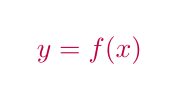
\begin{tikzpicture}
    \axes
    \fctn{purple,very thick}
    \node[purple,below right] at (5,-.5) {$y=f(x)$};
  \end{tikzpicture}
\end{center}
First of all, we can regard $f(x)$ itself as a differential form: one which simply does not use the variable $\dx$ (and thus takes the same value regardless of what $\dx$ is).
Thus, each little piece of the graph of this differential form will be a horizontal line, as shown below (we have included the graph of $f$ for comparison).
\begin{center}
  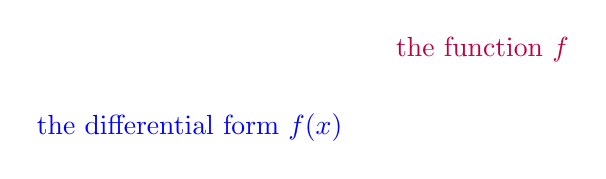
\begin{tikzpicture}
    \axes
    \fctn{dashed,purple}
    \node[purple,right] at (5,-.5) {the function $f$};
    \foreach \x/\y in \heights \draw[blue,very thick] (\x-.3,\y) -- (\x+.3,\y);
    \node[blue] at (2.5,-1.5) {the differential form $f(x)$};
  \end{tikzpicture}
\end{center}
This seems a little odd as a representation of $f$, so we may ask whether there is some differential form for which each piece of its graph looks like a corresponding part of the graph of $f$ itself.
Such a differential form is $f(x+\dx)$ --- since as $\dx$ varies around zero, $x+\dx$ varies around $x$.
\begin{center}
  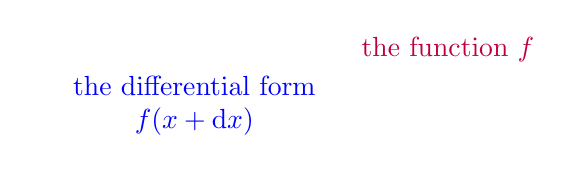
\begin{tikzpicture}
    \axes
    \fctn{dashed,purple}
    \node[purple,below right] at (5,-.5) {the function $f$};
    \foreach \x/\y in \heights {
      \begin{scope}
        \clip (\x-0.3,\y-0.3cm) rectangle (\x+0.3,\y+0.3cm);
        \fctn{blue,very thick}
      \end{scope}
    }
    \node[blue] at (3,-1.5) {\parbox{4cm}{\centering the differential form\\$f(x+\dx)$}};
  \end{tikzpicture}
\end{center}
Finally, consider the differential form $f(x+\dx)-f(x)$.
Its graph at $x$ looks just like a piece of the graph of $f$ near $x$, just as for the form $f(x+\dx)$, but now this graph is shifted down so that it crosses the $x$-axis at the point $(x,0)$ (this is what subtracting $f(x)$ accomplishes).
\begin{center}
  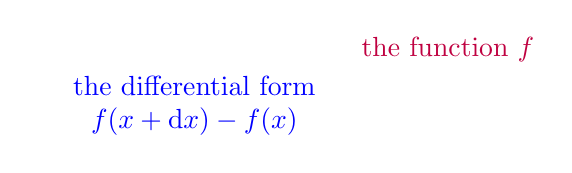
\begin{tikzpicture}
    \axes
    \fctn{dashed,purple}
    \node[purple,below right] at (5,-.5) {the function $f$};
    \foreach \x/\y in \heights {
      \begin{scope}
        \clip (\x-.3,-.3) rectangle (\x+0.3,.3);
        \fctn{blue,very thick,yshift=-\y}
      \end{scope}
    }
    \node[blue] at (3,-1.5) {\parbox{4cm}{\centering the differential form\\$f(x+\dx)-f(x)$}};
  \end{tikzpicture}
\end{center}
Note that the pieces of the graph of $f(x+\dx)-f(x)$ all look quite close to straight lines.
This happens whenever we ``zoom in'' sufficiently on a smooth function, and it is this observation that leads to the idea of differentiation.


\section{Differentials}
\label{sec:differentials}

In one-variable calculus, you may have encountered the differential of a function.
Namely, if $f$ is a function of one variable $x$, then its differential is
\begin{equation}
  \df = f'(x) \, \dx\label{eq:onevariable-differential}
\end{equation}
where $f'$ is the \emph{derivative} of $f$.
Note that $\df$ is a differential form.
Its graph looks like this (the function $f$ is the same one we were using as an example at the end of the last section).
\begin{center}
  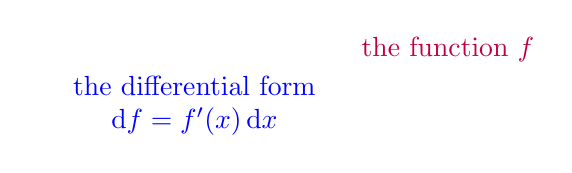
\begin{tikzpicture}
    \axes
    \fctn{dashed,purple}
    \node[purple,below right] at (5,-.5) {the function $f$};
    \foreach \x/\y/\slope in \heights {
      \begin{scope}
        \clip (\x-.3,-.3) rectangle (\x+0.3,.3);
        % \fctn{red,very thick,yshift=-\y}
        \draw[blue,very thick] (\x-.3,-\slope) -- (\x+.3,\slope);
      \end{scope}
    }
    \node[blue] at (3,-1.5) {\parbox{4cm}{\centering the differential form\\$\df = f'(x) \,\dx$}};
  \end{tikzpicture}
\end{center}
Note that this is barely distinguishable from the graph of $f(x+\dx)-f(x)$.
This is the whole point of the derivative: $f'(x)$ is the slope of the tangent line to the graph of $f$ at $x$, and that line is the best possible \emph{linear approximation} to the graph.
Indeed, recall that by definition, the derivative is
\[ f'(x) = \lim_{\dx\to 0} \frac{f(x+\dx)-f(x)}{\dx} \]
Thus, when $\dx$ is small, we can say that
\begin{equation}\label{eq:difference-quotient-close-derivative}
  \frac{f(x+\dx)-f(x)}{\dx}\quad\text{is very close to}\quad f'(x).
\end{equation}
Multiplying each of these by $\dx$, we find that
\begin{equation}
  f(x+\dx)-f(x) \quad\text{is very close to}\quad f'(x)\,\dx.\label{eq:difference-close-differential}
\end{equation}
This is what we saw in the above-remarked similarity of graphs.

\begin{adv}
  However, the quantities in~\cref{eq:difference-close-differential} are of a different order than those in~\cref{eq:difference-quotient-close-derivative}:
  $\frac{f(x+\dx)-f(x)}{\dx}$ and $f'(x)$ are zeroth order, while $f(x+\dx)-f(x)$ and $f'(x)\,\dx$ are first order.
  Thus, the precise meaning of ``close'' is different: in~\cref{eq:difference-close-differential} we mean that their difference is first-order, while in~\cref{eq:difference-quotient-close-derivative} we mean that their difference is second-order.
  This is why \cref{def:differential} below is phrased as it is.
\end{adv}

\Cref{eq:onevariable-differential} from one-variable calculus defines the \emph{differential} of $f$ in terms of the \emph{derivative} of $f$.
However, in multivariable calculus, it is more appropriate to do things in the other order, using the idea of~\cref{eq:difference-quotient-close-derivative} to define the differential \emph{first}, and then deducing a notion of ``derivative'' from this.

\begin{defn}\label{def:differential}
  If $f$ is a function of a point $\pt{x}$, then its \textbf{differential} is a linear differential 1-form $\df$ such that
  \[ f(\pt{x} + \dd\pt{x}) - f(\pt{x}) - \df \]
  is second order at $\pt{x}$.
  If such a form $\df$ exists, we say that $f$ is \textbf{differentiable} at $\pt{x}$.
\end{defn}

As always, we should explore a new definition with examples.

\begin{eg}
  Let $f(x) = x^2$, an ordinary one-variable function.
  Then
  \begin{align*}
    f(x + \dx) - f(x) &= (x+\dx)^2 - x^2\\
    &= x^2 + 2 x \, \dx + \dx^2 - x^2\\
    &= 2x \, \dx + \dx ^2.
  \end{align*}
  What linear form $\dd f$ can we subtract from this to make it second order?
  Recalling the rule for orders of polynomials, we may think of subtracting $2x \, \dx$, leaving the second-order term $\dx^2$:
  \[ f(x + \dx) - f(x) - 2x \, \dx \;=\; \dx^2. \]
  Thus, we have $\dd(x^2) = 2 x \, \dx$.
  Of course, this is the same result that we would have gotten from \cref{eq:onevariable-differential}.
\end{eg}

\begin{eg}
  Let $f(x,y) = x^2 + 2y^2 - xy$.
  Then
  \begin{align*}
    f(x+\dx,y+\dy) - f(x,y)
    &= (x+\dx)^2 + 2(y+\dy)^2 - (x+\dx)(y+\dy) - x^2 - 2y^2 + xy\\
    &= x^2 + 2 x \, \dx + \dx^2 + 2y^2 + 4y\,\dy + 2\dy^2\\
    & \hspace{2cm} - x^2 - x \, \dy - y \, dx - \dx \dy - x^2 - 2y^2 + xy\\
    &= 2x\,\dx + 4y\,\dy - x\,\dy - y\,\dx + \dx^2 + 2\dy^2 - \dx\,\dy\\
    &= (2x-y)\,\,dx + (4y-x)\,\dy + (\dx^2 + 2\dy^2 - \dx\,\dy)
  \end{align*}
  In the last line we have separated this into a linear form plus one of second order.
  Thus, we have
  \[ \dd(x^2 + 2y^2 - xy) = (2x-y)\,\dx + (4y-x)\,\dy .\]
\end{eg}

\begin{eg}
  Consider $f(x) = \sin x$.
  Using the sum identity for sine, we have
  \begin{align}
    \sin(x+\dx) - \sin (x)
    &= \sin x \cos \dx + \sin \dx \cos x - \sin x \notag\\
    &= \cos x \sin \dx + (\sin x) (\cos \dx - 1).\label{eq:sine-difference}
  \end{align}
  The usual way to proceed from here is to recall the limits
  \[ \lim_{h\to 0} \frac{\sin h}{h} = 1 \qquad\text{and}\qquad
  \lim_{h\to 0} \frac{\cos h - 1}{h} = 0 \]
  The second says exactly that the form $\cos \dx - 1$ is second-order.
  The first one implies that
  \[ \lim_{\dx\to 0} \frac{\sin \dx - \dx}{\dx} = 0 \]
  and therefore the form $\sin \dx - \dx$ is second-order.
  The ordinary functions $\cos x$ and $\sin x$, regarded as differential forms, are zeroth order; thus by the rules for orders, multiplying by them doesn't change the order.
  So we can write
  \begin{align*}
    \sin(x+\dx) - \sin (x)
    &= \cos x \sin \dx + (\sin x) (\cos \dx - 1)\\
    &= (\cos x )(\dx  + \sin \dx - \dx) + (\sin x) (\cos \dx - 1)\\
    &= \cos x \,\dx + (\cos x) (\sin \dx - \dx) + (\sin x) (\cos \dx - 1)
  \end{align*}
  which is written as the linear form $\cos x \,\dx$ plus a second-order one.
  Thus, $\dd(\sin x) = \cos x \,\dx$.

  Another, perhaps more intuitive, way to proceed from \cref{eq:sine-difference} is to recall the power series expansions
  \begin{align*}
    \sin x &= x - \frac{x^3}{3!} + \frac{x^5}{5!} - \cdots\\[2pt]
    \cos x &= 1 - \frac{x^2}{2!} + \frac{x^4}{4!} - \cdots
  \end{align*}
  Therefore, we have
  \begin{align*}
    \sin \dx - \dx &= - \frac{\dx^3}{3!} + \frac{\dx^5}{5!} - \cdots\\[2pt]
    \cos \dx - 1 &= - \frac{\dx^2}{2!} + \frac{\dx^4}{4!} - \cdots
  \end{align*}
  so the rules for orders of polynomials say that the first is third-order (hence also second-order) and the second is second-order.
  This does require knowing that the rules for orders of polynomials also apply to power series, but this is true.
  (A deeper problem is that when calculating the power series expansions of sine and cosine in one-variable calculus, you probably used the fact that you already knew their derivatives.)
\end{eg}

A convenient way to work with differentials is to introduce the notion of ``approximation to first order''.

\begin{defn}
  We say that two differential forms $\omega$ and $\eta$ are \textbf{equal to $n\th$ order} if their difference $\omega-\eta$ is $(n+1)\st$ order.
  In this case we write
  \[\omega\apx{n} \eta.\]
\end{defn}

For example, we have $x\,\dx + \dx^2 \apx1 x\,\dx - e^x \,\dx^2$, since their difference is
\[ (x\,\dx + \dx^2) - (x\,\dx - e^x\, \dx^2) = (1+e^x)\dx^2 \]
which is second order.

The relation $\apx{n}$ behaves roughly like equality.
For instance, we can add or subtract the same differential form from both sides.
We can also multiply both sides by any continuous differential form, since multiplying by a zeroth order form doesn't change the order.
Finally, we can of course discard any terms of greater than $n\th$ order from an $n\th$-order approximate equality.

Now we can equivalently state the definition of a differential: $\df$ is a linear differential 1-form such that
\[ f(x+\dx) \apx1 f(x) + \df, \]
if such exists.
Our previous calculations of differentials can all be written in this way.
For instance,
\begin{align*}
  (x+\dx)^2 &= x^2 + 2 x\,\dx + \dx^2\\
  &\apx1 x^2 + 2 x\,\dx
\end{align*}
since $\dx^2$ is second order.
Therefore, $\dd(x^2) = 2x\,\dx$.

We can also deduce all the usual derivative rules, written in terms of differentials.
For instance, given functions $f$ and $g$, consider their sum $f+g$.
\begin{align*}
  f(x+\dx) + g(x+\dx)
  &\apx1 f(x) + \df + g(x) + \dg\\
  &= \big[f(x) + g(x)\big] + \big[ \df + \df \big]
\end{align*}
Thus, we have
\[ \dd(f+g) = \df + \dg. \]
Similarly, for the product rule, we compute
\begin{align*}
  f(x+\dx) \, g(x+\dx)
  &\apx1 \big(f(x)+\df\big)\big(g(x) + \dg \big)\\
  &= f(x) g(x) + f(x) \,\dg + g(x) \,\df + \df\,\dg\\
  &\apx1 f(x) g(x) + f(x) \,\dg + g(x) \,\df
\end{align*}
since $\df\,\dg$ is a product of two first-order forms, hence second-order.
Thus,
\[ \dd(f\,g) = f\,\dg + g\,\df.\]
% TODO: Chain rule

Importantly, these same rules apply to functions of more than one variable.

\begin{eg}\label{eg:twovar-differential}
  If $f(x,y) = x^2y + xy^2$, then we can use the sum and product rules to obtain
  \begin{align*}
    \dd(x^2y + xy^2) &= \dd(x^2y) + \dd(xy^2)\\
    &= x^2\,\dy + y \,\dd(x^2) + x \,\dd(y^2) + y^2\,\dx\\
    &= x^2\,\dy + y \,(2x\,\dx) + x\, (2y\,\dy) + y^2\,\dx\\
    &= (2xy + y^2)\,\dx + (x^2+2xy)\,\dy
  \end{align*}
\end{eg}

\section{Differential forms versus vectors}
\label{sec:forms-vs-vectors}

% TODO: Transposes
% TODO: Gradient = transpose of differential

\section{Derivatives}
\label{sec:derivatives}

We can now define the \emph{derivative} in terms of the \emph{differential}.
Note that in one dimension, a linear differential 1-form must be of the form
\[ g(x) \,\dx \]
for some function $g$.
In particular, if $f$ is a differentiable function of one variable $x$, then $\df = g(x) \, \dx$ for some function $g$, which we call the \emph{derivative} of $f$ and denote by $f'$.
In other words, $\df = f'(x)\,\dx$ (this is \cref{eq:onevariable-differential}), or
\[ f'(x) = \frac{\df}{\dx}. \]
This is a notation that you have probably seen before.
The point is that now, we have given separate meanings to $\dx$ and $\df$, and \emph{defined} $f'(x)$ to be their quotient.

However, when there is more than one variable, this doesn't work any more!
For instance, consider the function $f(x,y) = x^2y + xy^2$, whose differential we found in \cref{eg:twovar-differential} to be
\[ \df = (2xy + y^2)\,\dx + (x^2+2xy)\,\dy.\]
Since there are two variables $x$ and $y$, there are two differentials $\dx$ and $\dy$ appearing in this expression for $\df$.
Thus, we can no longer simply divide $\df$ by $\dx$ to get a simple function.
We could of course write
\begin{align*}
  \frac{\df}{\dx} &= (2xy + y^2) + (x^2+2xy)\frac{\dy}{\dx} \qquad\text{or}\\[2pt]
  \frac{\df}{\dy} &= (2xy + y^2)\frac{\dx}{\dy} + (x^2+2xy)
\end{align*}
but in neither case is the right-hand side an ordinary function of $x$ and $y$.
We conclude that
\begin{center}
  \fbox{\emph{It makes no sense to talk of ``the'' derivative of a function of more than one variable!}}
\end{center}
However, we do have two ordinary functions that have about an equal claim to be called a ``derivative'' of our function $f$ above, namely $2xy + y^2$ and $x^2+2xy$.
Neither one ``tells the whole story'' about the differential $\df$ on its own, but together they do.
Thus, we refer to each of them as a \emph{partial derivative} of $f$.

\begin{defn}
  If $f$ is a differentiable function of two variables $x,y$, then its \textbf{partial derivatives} are the functions $\pder{f}{x}$ and $\pder{f}{y}$ such that
  \[ \df = \pder{f}{x}\,\dx + \pder{f}{y}\,\dy\]
  Similarly, if $f$ is a differentiable function of three variables $x,y,z$, then its partial derivatives $\pder{f}{x}$, $\pder{f}{y}$, and $\pder{f}{z}$ are the functions such that
  \[ \df = \pder{f}{x}\,\dx + \pder{f}{y}\,\dy + \pder{f}{z}\,\dz.\]
\end{defn}
The symbol $\partial$ is a stylized ``$d$'' and is pronounced either ``del'' or ``partial''.
Note that unlike for ordinary one-variable derivatives, the symbols $\partial f$ and $\partial x$ have \emph{no meaning} on their own.

\begin{eg}
  For the function $f(x,y) = x^2y + xy^2$ with $\df = (2xy + y^2)\,\dx + (x^2+2xy)\,\dy$, we have
  \begin{align*}
    \pder{f}{x} = 2xy + y^2 \qquad\text{and}\qquad
    \pder{f}{y} = x^2+2xy.
  \end{align*}
\end{eg}

% TODO: Directional derivatives
% TODO: Geometrical interpretation

\end{document}
